%%%%%%
%
% $Autor: ter Veen $
% $Datum: 01.06.2024 $
% $Version: 1 $
% $Pfad: SchrittmotorArduino/DevoloperDoc/tikz/ArduinoPinout.tex $
%
%%%%%%

% Für schnelle Anpassungen
%\documentclass[12pt,a4paper]{scrbook}
%\usepackage{tikz}
%\usetikzlibrary{shapes,arrows.meta,positioning}
%\begin{document}
	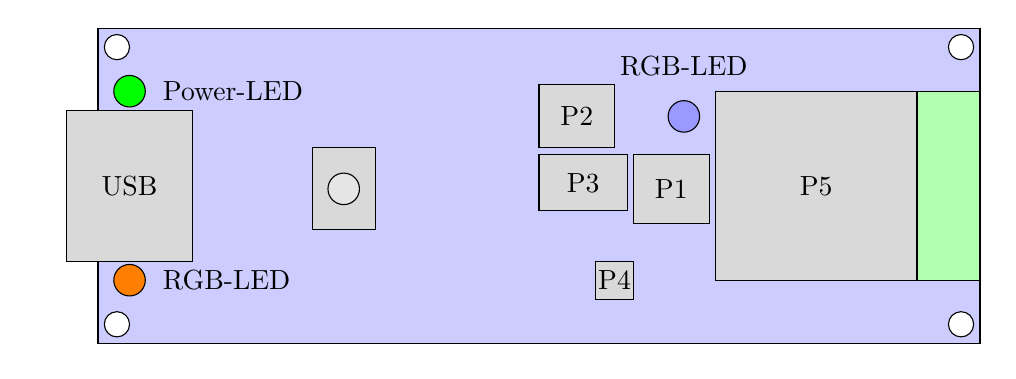
\begin{tikzpicture}[scale=0.8]
		% Arduino Dummy
		\draw[fill=blue!20] (1,0) rectangle (15,5);
	
		% Module
		\draw[fill=gray!30] (10.8,1) rectangle (14,4) node[pos=0.5, align=center] {P5};
		\draw[fill=green!30] (14,1) rectangle (15,4) node[pos=0.5, align=center] {};
		\draw[fill=gray!30] (0.5,1.3) rectangle (2.5,3.7) node[pos=0.5, align=center] {USB};
		\draw[fill=gray!30] (9.5,1.9) rectangle (10.7,3) node[pos=0.5, align=center] {P1}; % Mikrophone
		\draw[fill=gray!30] (8,3.1) rectangle (9.2,4.1) node[pos=0.5, align=center] {P2}; % IMU
		\draw[fill=gray!30] (8,2.1) rectangle (9.4,3) node[pos=0.5, align=center] {P3}; %  Näherungs-,Umgebungslicht-, Farb- und Gestensensor
		\draw[fill=gray!30] (8.9,0.7) rectangle (9.5,1.3) node[pos=0.5, align=center] {P4}; % Drucksensor
		\draw[fill=gray!30] (4.4,1.8) rectangle (5.4,3.1) node[pos=0.5, align=center] {};
		\draw[fill=gray!20] (4.9,2.45) circle (0.25) node[pos=0.5, align=center] {};
		
		% Bohrlöcher
		\draw[fill=white] (1.3,0.3) circle (0.2) node[right=1mm]{};
		\draw[fill=white] (1.3,4.7) circle (0.2) node[right=1mm]{};
		\draw[fill=white] (14.7,0.3) circle (0.2) node[right=1mm]{};
		\draw[fill=white] (14.7,4.7) circle (0.2) node[right=1mm]{};
		
		% LED´s
		\draw[fill=green] (1.5,4) circle (0.25) node[right=3mm] {Power-LED};
		\draw[fill=orange] (1.5,1) circle (0.25) node[right=3mm] {RGB-LED};
		\draw[fill=blue!40] (10.3,3.6) circle (0.25) node[above=4mm] {RGB-LED};
		
	\end{tikzpicture}
%\end{document}